\title{\vspace{160px} \textbf{\huge{Multimedia}} \\\vspace{17.5px} \LARGE{Homework 1}  \vspace{10px}}
\author{\href{https://github.com/imAlessas}{Alessandro Trigolo}}
\date{30 Aprile 2024}

\begin{document}

\maketitle\newpage




\section{Obiettivo}
\todo{Descrivi decentemente l'obiettivo}



\section{Codice sorgente}
\todo{Rifai introduzione}
Il linguaggio scelto per completare le richieste dell'homework è \texttt{Python}; all'interno del documento saranno presenti solo i punti salienti dello script, che comunque può essere ispezionato al seguente \href{https://github.com/imAlessas/computer-networks/blob/main/multimedia/hw-1/script/lossless_coding.py}{\texttt{link}}.


\subsection*{Task 1}

La prima richiesta dell'homework era divisa in due macro parti, la prima era quella di selezionare e mostrare un'immagine mentre la seconda richiesta chiedeva di calcolare l'entropia dell'immagine.

L'immagine scelta è un'immagine di \textsl{Spider-Man} a colori, di conseguenza è necessario estrarne la luminaza per fara diventare in binaco e nero. Dopo aver caricato l'immagine a colori con l'opportuna funzione \texttt{imread} del pacchetto \texttt{matplotlib.image} è necessario usare la funzione \texttt{cvtColor} del pacchetto \texttt{cv2} di \texttt{opencv}. Il seguente script, dopo aver eseguito le suddette operazioni si occupa di mostrare le due immagini a schermo attraverso una \texttt{subplot}.

\begin{lstlisting}
# Prepare to load the image
img_file_name = "spiderman"
img_extension = ".jpg"
current_dir = os.getcwd()

# path to reach the img
path_to_img = os.path.join(current_dir, "multimedia", "hw-1", "script", "imgs") + "/"

# loads the colored image
img = mpimg.imread(path_to_img +  img_file_name + img_extension) 

# extracts the luminance
gray_img = cv2.cvtColor(img, cv2.COLOR_BGR2GRAY)

# creates a figure with two subplots
fig, axs = plt.subplots(1, 2, figsize=(12, 6))

# displays the colored image in the first subplot
axs[0].imshow(img, cmap='gray')
axs[0].set_title('Colored image')
axs[0].axis('off')

# displays the grayscale image in the second subplot
axs[1].imshow(gray_img, cmap='gray')
axs[1].set_title('Grayscale image')
axs[1].axis('off')

plt.show()
\end{lstlisting}

\noindent Dopo aver eseguito lo script soprastante si può notare che la luminanza dell'immgine è stata estratta con successo (figura \ref{fig:luminanza}).

\begin{figure}
    \centering
    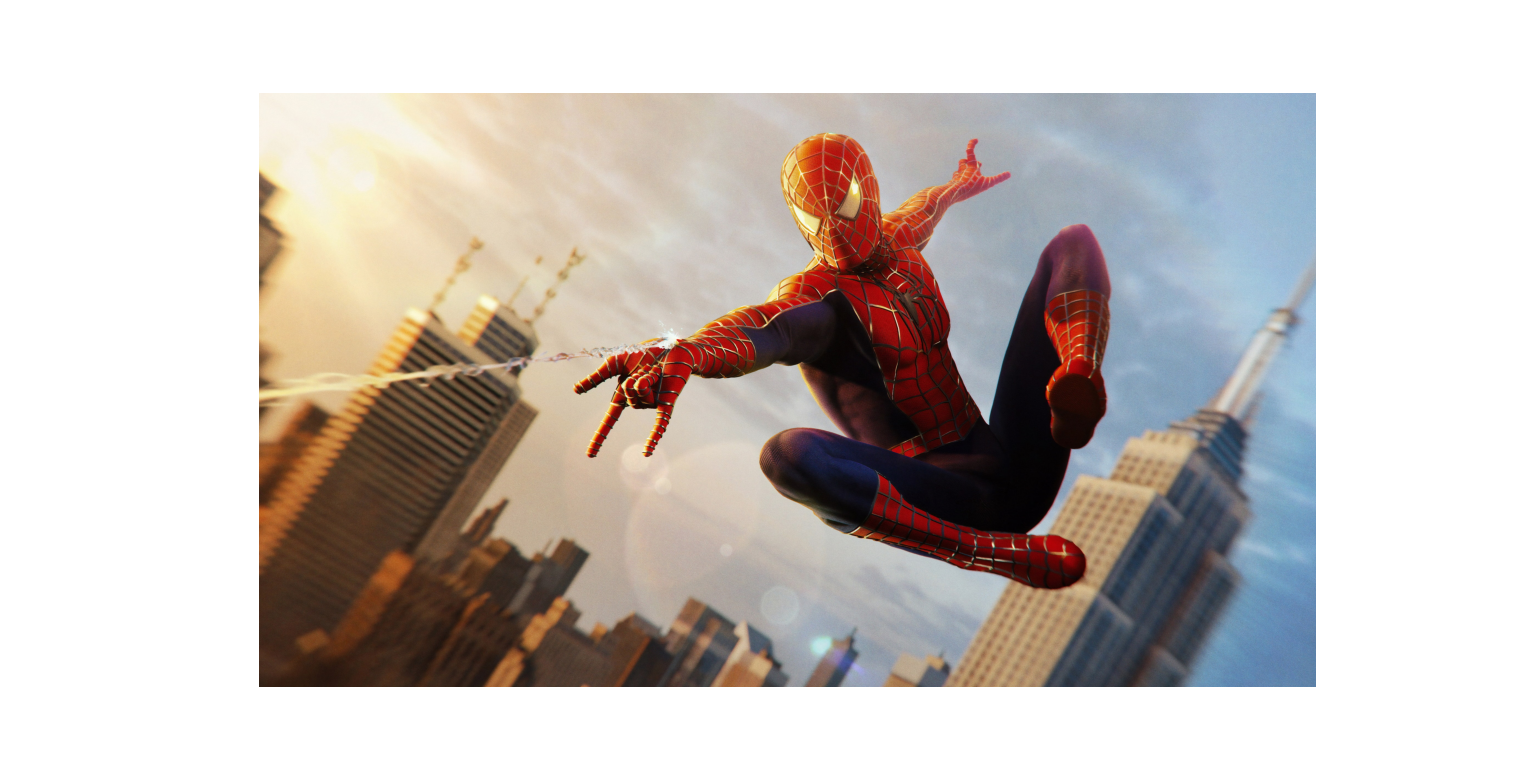
\includegraphics[width = .7\textwidth]{hw-1/report/imgs/colored.png}
    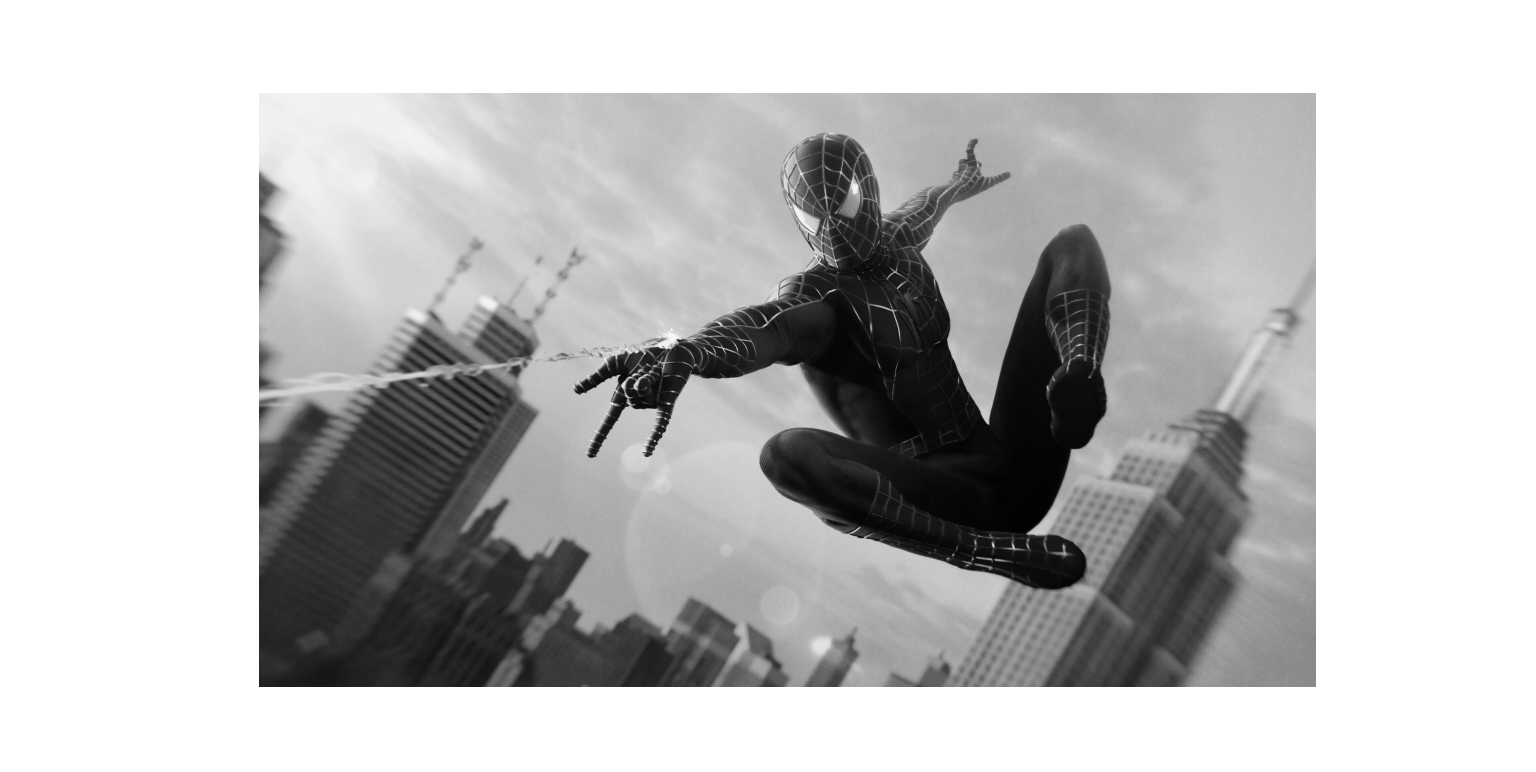
\includegraphics[width = .7\textwidth]{hw-1/report/imgs/grayscale.png}
    \caption{Estrazione della luminaza da una immagine a colori.}
    \label{fig:luminanza}
\end{figure}

\FloatBarrier\noindent In secondo luogo è necessario calcolare l'entropia dell'immagine in bianco e nero. L'entropia di di un'immagine, ma in genere di qualsiasi tipo di sorgente (o meglio, variabile aleatoria $X$), è un numero che indica l'\textbf{informazione media} ed è definita come segue:

\begin{gather*}
    H(X) = E[I(X)] \, = \, \sum_{i = 1}^M p_i\log_2\left( \frac{1}{p_i} \right)
\end{gather*}

\noindent Dove con $M$ si indica il numero di elementi nell'insieme $X$ e con $p_i$ si indica la probabilità di accadere dell'elemento \textit{i}-esimo della variabile aleatoria $X$. Questa formula si riassume nel seguente script, dove l'immagine viene trasporta e convertita in un vettore di pizel monodimensionale. In secondo luogo attraverso la funzione \texttt{numpy.histogram} si contano il numero di occorrenze per ogni valore di pixel. Infine, per calcolare la probabilità, si divide il numero di occorrezze per il numero totale di occorrenze, escludendo eventuali valori diversi da zero.


\begin{lstlisting}
# flatten the transposed matrix to read pixels row by row
rasterScan = np.transpose(gray_img).flatten()

# count the occurrences of each pixel value
occurrencies = np.histogram(rasterScan, bins=range(256))[0]

# calculate the relative frequencies
p = occurrencies / np.sum(occurrencies)

# remove zero-values of probability
p = p[p > 0]

# compute and display the entropy
HX = - np.sum(p * np.log2(p))
print(f"\nThe entropy of {img_file_name} is {HX:.3f} bpp\n")
\end{lstlisting}

\noindent Dopo aver eseguito lo script si ottiene che l'entropia dell'immagine scelta è di circa \textbf{7.530 bpp}.


\subsection*{Task 2}
La seconda task richiedeva di utilizzare una compressione a dizionario, come \texttt{zip} nel caso di \textsl{Windows} per poi calcolare il bitrate risultante. Lo script necessario per soddisfare la richiesta è presentato nel frammento di codice sottostante. In particolare le prime due righe si occupano di \textsl{zippare} il file mentre le seguenti si occupano di ottenere la dimensione dell'immagine compressa. Infine nelle ultime righe si calcola l'effettivo \textsl{bitrate} dividendo la dimensione del file compresso con \todo{capisci cosa mettere qui}

\begin{lstlisting}
# zip the image
cmd = f"zip {path_to_img}{img_file_name}.zip {path_to_img}{img_file_name}.jpg"
os.system(cmd)

# get the zip bytes
img_stats = os.stat(f"{path_to_img}{img_file_name}.zip")
zip_bytes = img_stats.st_size

# get the birate
zip_bitrate = zip_bytes * 8 / (512 * 512) 

print(f"\nThe bitrate of {img_file_name}.zip is {zip_bitrate:.3f} bpp\n")
\end{lstlisting}

\noindent Dopo aver eseguito lo script si ottiene quindi il valore del bitrate che corrisponde a \todo{sistema}





\subsection*{Task 3}

\section{Conclusioni}

\end{document}
